\subsection{Data selection and $\gamma$-ray flux extraction}

We use $\sim9$ years (7 Aug 2008 - 16 Oct 2017) of the latest version
(P8R2 ULTRACLEANVETO V6) of the LAT's photon data between 10 GeV to 1 TeV.
We observe $\gamma$ rays from the Earth's thin upper atmosphere by selecting the
nadir angle ($\theta_{\rm NADIR}$) from $68.4^\circ$ to $70.0^\circ$ \cite{previouswork} as
demonstrated in figure~\ref{gamma_production_schematic}. The incidence angle cut,
$\theta_{\rm LAT}<70^\circ$, is also applied.

% \begin{figure}[h!]
%     \centering
%     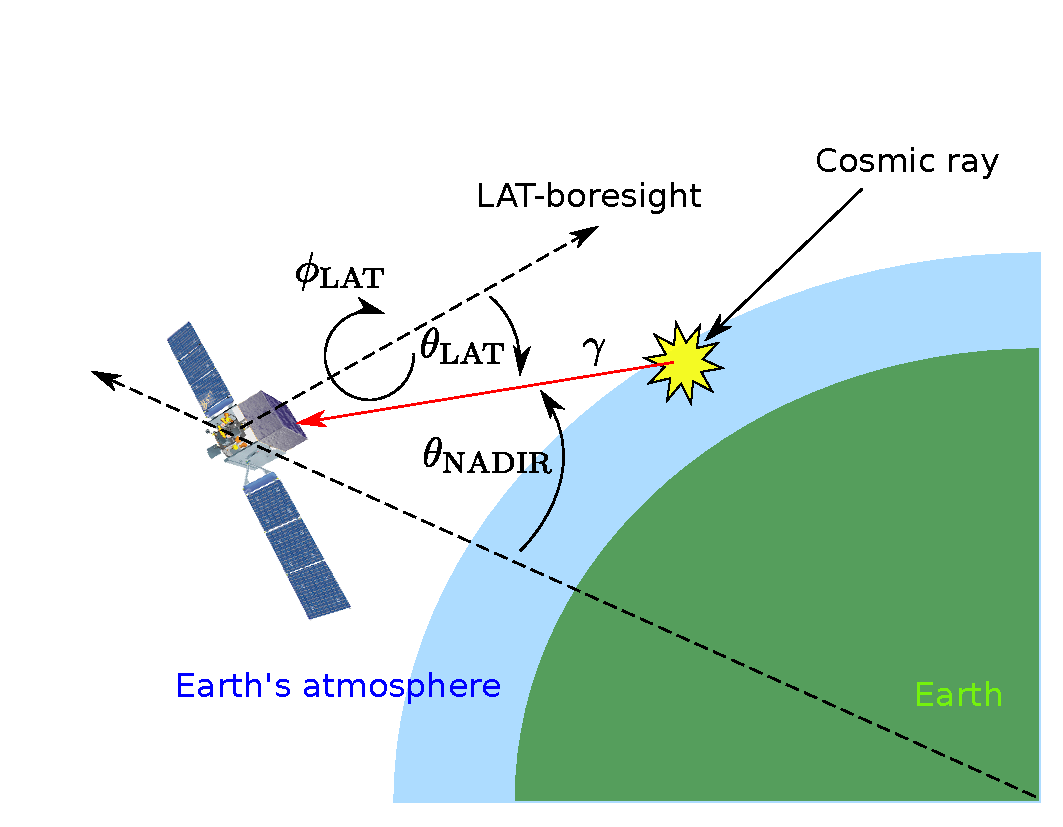
\includegraphics[width=0.5\textwidth]{img/gamma_production_schematic}
%     \caption{Schematic of $\gamma$-ray production}
%     \label{gamma_production_schematic}
% \end{figure}

% \begin{wrapfigure}{r}{0.5\textwidth}
%     \begin{center}
%         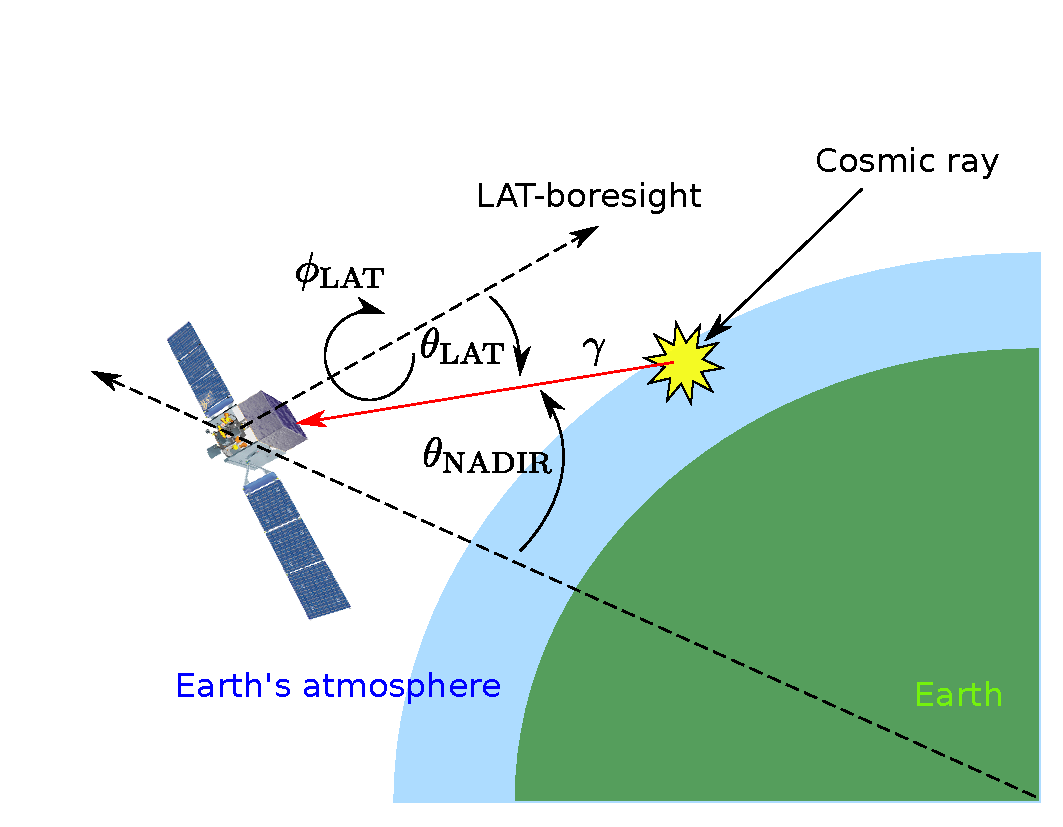
\includegraphics[width=0.5\textwidth]{img/gamma_production_schematic}
%     \end{center}
%     \caption{Schematic of $\gamma$-ray production}
%     \label{gamma_production_schematic}
% \end{wrapfigure}

\begin{figure}[h]
    \begin{minipage}{0.45\textwidth}
        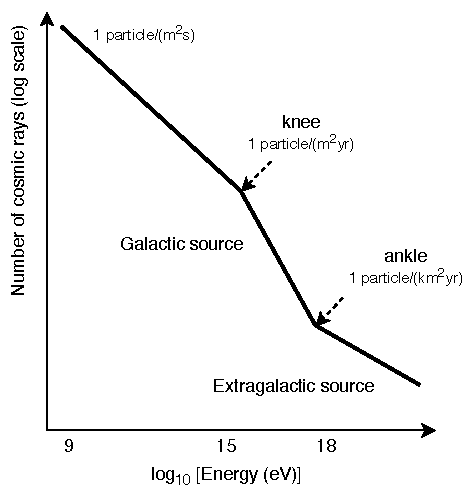
\includegraphics[width=\textwidth]{img/CRs_overview}
        \caption{All-particle CR spectrum.}
        % \caption{The all particle spectrum of cosmic rays, image taken from }
        \label{cr_knee_ankle}
    \end{minipage}\hspace{2pc}
    \begin{minipage}{0.55\textwidth}
        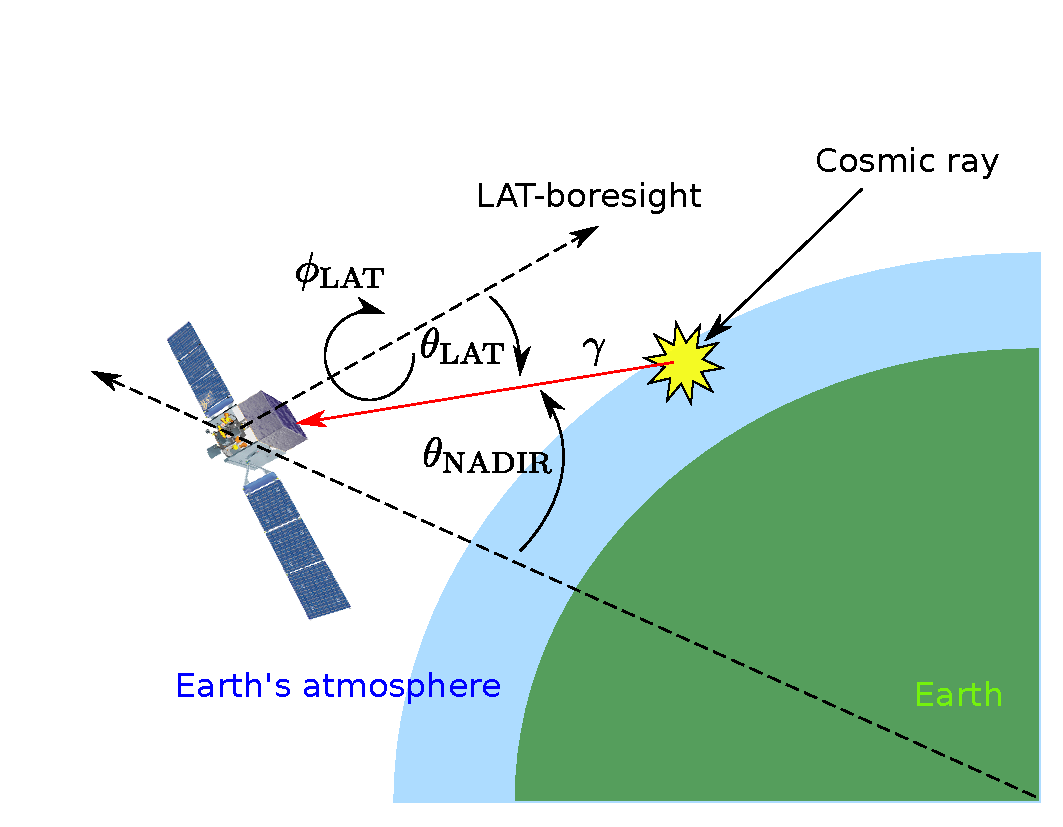
\includegraphics[width=\textwidth]{img/gamma_production_schematic}
        \caption{Schematic of high-energy Earth's $\gamma$-ray production.}
        \label{gamma_production_schematic}
    \end{minipage} 
\end{figure}

% The observed flux is defined as differential flux where the governing equation
% for the calculation is represented as equation (\ref{flux_definition})
The observed flux for a given energy bin is calculated using
\begin{equation}
    \textbf{Flux} \equiv \frac{dN_\gamma}{dE} = \frac{\int_{\textrm{Limb region}}(\textrm{Count map}/\textrm{Exposure map})}{\Delta\Omega\Delta E }
    .\label{flux_definition}
\end{equation}

% Where count map is filled up with selected $\gamma$-ray and 
Here the count map is filled with numbers of photons, the exposure map represents 
the exposure time as well as the effective area of spacecraft 
which is a function of energy and $\theta_{\rm LAT}$, $\Delta E$ is the energy bin width,
and $\Delta\Omega$ is the solid angle of the thin-target Earth's limb region.
% Procedure of computation is begin with the requirement of 25 bins of histogram of
% the $\gamma$-ray flux which contain a various median of energy in each bin.
We perform the analysis with 25 bins of energy, equally spaced in logarithmic scale.
% Consequently, the number of count map and exposure map will be exactly the same as
% the energy bins. The calculation of exposure map is done by using log file of the
% spacecraft combine with the responsiveness of the spacecraft which has to be consider
% in every step time while spacecraft is online. 
For a given energy bin, the exposure map is calculated using the spacecraft's position
and orientation recorded in 30-second time steps, each of which involves a complex
coordinate transformation to create a map in the zenith-azimuth system.
Such computationally intensive task requires parallel
processing with Master-Slave technique that we have developed.
% which cause a huge amount of computing process.
% That is the reason why paralleling processing with Master-Slave technique is
% applied in this work.


\subsection{Interaction model}
In this work, we test 2 models of CR protons: single-power law (SPL) model
containing one spectral index, and broken-power law (BPL) model containing two
spectral indices with a break energy.

% The model for a scattering amplitude from hadronic collision \cite{K&Omodel}
% that could produce a photon as a secondary product which could be
% detected by \textit{Fermi}-LAT as equation \ref{eq:interaction_model}.

% According to \cite{K&Omodel}, Earth's limb photon are mainly came from proton-proton
% collisions via hadronic interaction where the neutral pions was produced
% and decays into a pair of photons. The secondary photon spectrum could be summarized by
Earth's limb photons above ~500 MeV are mainly from the hadronic
interactions of proton-air collisions, producing neutral pions
which quickly decay into pairs of $\gamma$-ray photons. According to \cite{K&Omodel},
the secondary photon spectrum could be summarized by

\begin{equation}
    \frac{dN_\gamma}{dE_\gamma}\propto \int^{E_{\text{max}}}_{E_\gamma} dE'\frac{dN_p}{dE'} \frac{d\sigma^{pp\rightarrow\gamma}(E',E_\gamma)}{dE_\gamma}
    ,\label{eq:interaction_model}
\end{equation}
where here $dN_\gamma/dE_\gamma$ is the measured Earth's limb $\gamma$-ray spectrum,
$dN_p/dE'$ is the CR proton model, and $\sigma^{pp\rightarrow\gamma}$ is the interaction
cross section.
We take into account the contribution from CR He particles to the production of secondary
photons by using the cross section ratio ($\sigma_{\rm HeN}/\sigma_{p\rm N}$) from
\cite{WAtwater} and the He spectrum measurement by \cite{AMS-02Helium}. This modifies
equation~(\ref{eq:interaction_model}) to
% For the real use case, the interaction of an alphaparticle with the air
% has a significant contribution to the secondary photon.
% A modification of He-air interaction could be
% applied by using a fraction of cross-section from a given atomic number
% \cite{WAtwater}. The helium spectrum in rigidity is taken from the real
% measurement \cite{AMS-02Helium}. Then the input of the modified model
% is left only a proton spectrum.

\begin{equation}
    \frac{dN_{\gamma}}{dE_\gamma}(E_\gamma) \propto
    \sum_{E'_i}\left[\frac{E'_i}{E_{\gamma}}\Delta(\ln E'_i) \right]
    \left[ 
        f_{pp}\frac{dN_p}{dE'_i}
        \left\{
            1+\frac{\sigma_{\text{HeN}}}{\sigma{p\rm N}}\left(\frac{dN_p}{dR}\right)^{-1} \frac{dN_{\text{He}}}{dR} \frac{dR_{\text{He}}}{dR_p} 
        \right\}
    \right]
    ,\label{eq:derived_model}
\end{equation}
where $f_{pp} \equiv E_\gamma(d\sigma^{ij\rightarrow\gamma}/dE_\gamma)$
is the interaction cross section table in \cite{K&Omodel}.

\subsection{Optimization}

We use the SPL and BPL models for $dN_p/dE'$ in equation~(\ref{eq:derived_model}) and vary their parameters
(normalization, spectral indices, break energy) so that the resulting $dN_\gamma/dE_\gamma$
from the model fits to the measured Earth's limb $\gamma$-ray spectrum with maximum
likelihood. We employ the particle swarm optimization (PSO) \cite{pso_optimize} as our fitting algorithm
because PSO is efficient at avoiding local maxima and reaching the global maximum in
this multi-parameter problem.
% For the hyper parameter setting, we spawn 50 states of
% the particle in parameter space where it randomly be initialized from a spectral
% indices between 2.5 to 3.0 as well as minimum and maximum breaking energy of BPL are
% 310 and 350 GeV. The iteration process of the optimization will stop when standard deviation
% from log-likelihood of every particles less than 0.1 since the assumption is the 
% particle will locate at around the same position in parameter space when it reach the 
% global minimum and yield a similar profits.
For the setting, we spawn 50 states of particles in hyper parameter space
in which the states are randomly initialized with the spectral indices
between 2.5 and 3.0, as well as the minimum and maximum breaking energy of BPL
between 310 and 350 GeV. The optimization iteration process stops when the
standard deviation of the log-likelihood of each particle is less than 0.1
since the particles would locate at around the same position in the parameter
space when the optimization reaches the global minimum and yields similar profits.

% Optimizing a problem with multiple parameters might cause a local minimum
% which will cause an early stopping of the optimization proces before 
% reaching to the global minimum. In this work, a simple gradient optimization
% with a set of different initial values yield a various output which implicitly
% imply that there are local minimum exists in this problem. 
% To get rid of the local minimum, particle swarm optimization (PSO) is applied
% to find the best fit parameters \cite{pso_optimize}.



